\subsection{About GROMOS software}\label{subsec:about_}
GROMOS is an acronym of the \textbf{GROningen MOlecular Simulation} computer program. It's a software package used for computer simulations of molecular systems like proteins, inorganic and organic chemical compounds, DNA, etc, developed since 1978 and it is written in C++ programming language.
In order to preform MD simulations with GROMOS software, three main elements must be generated and used in every step of the simulation. They are:
\begin{itemize}
    \item Topology of the system (\textbf{*.top} file)
    \item Spacial coordinates of the system (\textbf{*.cnf} file)
    \item Input file (\textbf{*.imd} file) with the parameters for the MD simulation
\end{itemize}

\subsubsection{Building a topology}
The first task is to generate a molecular topology file containing the topological and force-field data concerning the molecular system under consideration. The topology information is referred to the data on the covalent structure, atomic masses, charges, van der Waals parameters, atom-atom distance restraints specification, restraints specification, local-elevation dihedral angles specification, etc. Every constant and parameter described in section \ref{subsec:FF} it's contained in the \textbf{*.top} file. In GROMOS, a molecular topology is generated from molecular topology building blocks which carry the topological information of molecules like amino acid residues, nucleotides, etc. The molecular topology
building blocks can be linked together into a complete molecular topology file using the GROMOS++ program \texttt{make\_top}. In this work, the \textbf{GROMOS-54a7} force-field was selected to preform the molecular dynamics simulations. 

\subsubsection{Generating atomic cartesian coordinates}
The next step is to generate the configurational information regarding to the atomic coordinates and atomic coordinate dependent or related quantities, such as velocities and forces, atom-atom distances, dihedral angles, energies, size of the computational box, etc. These two types of information (topologycal and configurational) are generally stored in separate files, since configurations change continuously during a simulation, whereas molecular topological data generally do not change.

Coordinates for biomolecules are often available from X-ray or Nuclear magnetic resonance spectroscopy (NMR) experiments and can be obtained in Protein Data Bank (PDB) format, which can be converted to GROMOS format using the GROMOS++ program \texttt{pdb2g96}. In this case, the \textbf{*.pdb} files for both alanines configurations (extended and helix) are generated using VMD's plugin \texttt{Molefacture} which is a user interface to create and edit molecules. This includes the ability to add, delete, or manipulate their structure at an atomic level, and to build new components from a library of common fragments.
As the coordinates for hydrogen atoms are not present in \textbf{*.pdb} files (usually) they have to be generated using the GROMOS++ program \texttt{gch}. In the standard GROMOS force fields, part of the hydrogen atoms (polar, aromatic) are explicitly treated, whereas other hydrogen atoms (aliphatic, some aromatic) are implicitly treated by incorporation into the (carbon)atom to which they are attached. Program \texttt{gch} calculates optimal positions for hydrogen main structure atoms.

\subsubsection{Energy minimisation of the peptide}
Before putting any peptide into a box of solvent, its configuration has to be relaxed by energy minimisation. The use of this technique with an empirical energy function such as Equation \ref{eq:v_general} is a widely used tool for obtaining low-energy configurations of a molecular system. In this work, the \textit{steepest descent method} is implemented for this propose \cite{van1988role}.
When applying energy minimization algorithms one searches for a minimum energy configuration of a system by moving (approximately) along the direction of the gradient of the potential energy through configuration space.
\begin{equation}
    \Delta r_i \sim -\frac{\delta }{\delta r_i}V(r_1,r_2,...,r_n)
    \label{eq:gradient}
\end{equation}
where $\Delta r_i$ is the change in position, $V$ the potential energy function given by Equation \ref{eq:v_general}, and $r_i$ the position vector of a particle $i$. 

Since all configurations used for simulations were not directly obtained from physical data, but instead generated with VMD, these artificial structures can possess high amounts of potential energy so they were minimized with a maximum minimization time of 5 [$ps$] in 2 [$fs$] steps (maximum time because the simulation also stops if the potential energy difference between two steps is less than a certain minimum, in this case 0.1 [$kJ/mol$])

\subsubsection{Solvating the peptide}\label{subsubsec:sim_box}
Once the structure is minimized, the next step is to put the peptide in a box of solvent using the GROMOS program \texttt{sim\_box} which can solvate the solute in a pre-equilibrated box of solvent molecules. There are three types of box's shapes (rectangular, truncated octahedron and cilindrical), and a water model must be determined. In this work, the rectangular box shape and a SCP-water model was selected to perform the simulations. 

In order to relax the unfavorable atom-atom contacts between the solute and the solvent, energy minimisation of the solvent should be performed while keeping the solute positionally restrained (i.e. connecting the atom to a reference position by a spring). The restraining is achieved by a harmonic force term with a force constant determined in the simulation input file (\textbf{*.imd}). 
\begin{figure}[h]
    \centering
    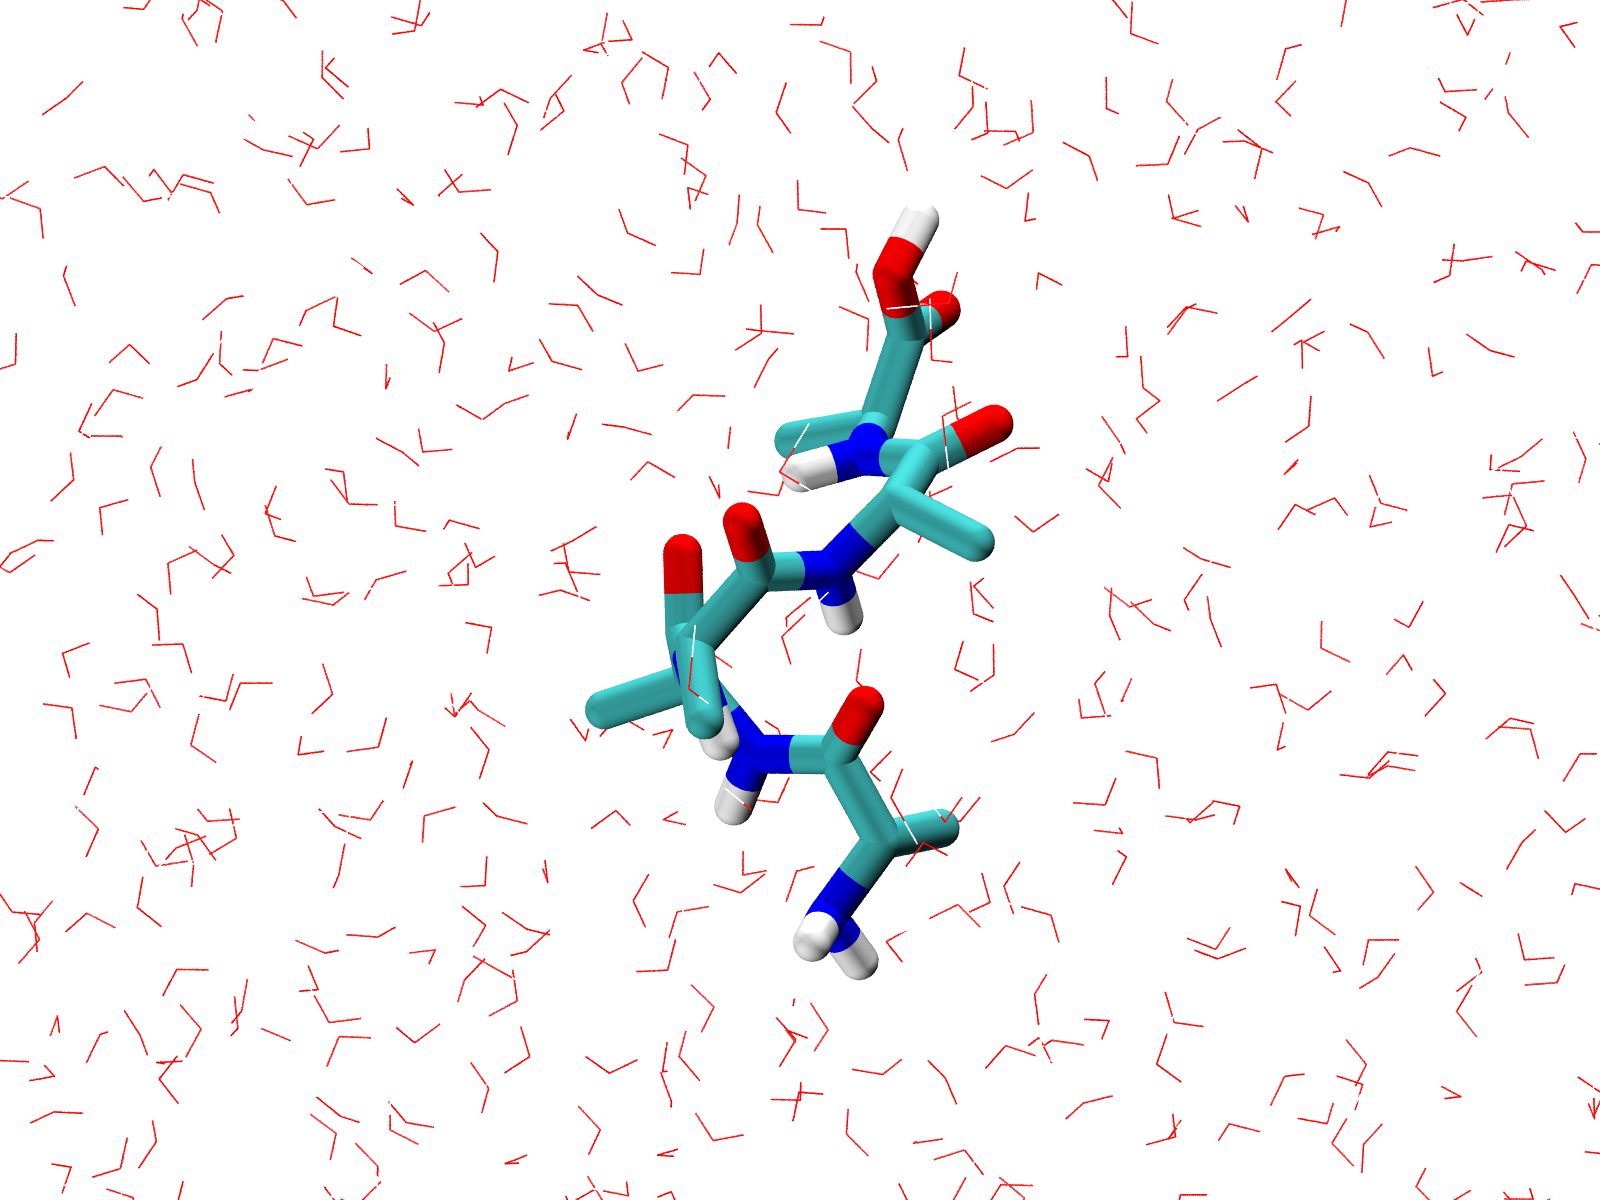
\includegraphics[scale=0.18]{Figures/Chapter_5/sim_box.png}
    \caption{Penta-alanine in box full of water molecules.}
    \label{fig:sim_box}
\end{figure}

\begin{table}[th] %th for exact position.
    \centering
    \begin{tabular}{c|cc|cc}
    \toprule
    \multirow{2}{4em}{n-ALA}           &   \multicolumn{2}{c|}{\textbf{Helix}} & \multicolumn{2}{c}{\textbf{Extended}}\\

    &   Box size $[nm^3]$ & $N^o$ atoms    &   Box size $[nm^3]$     &   $N^o$ atoms\\
    \midrule
    1         &   2.879  &   2310                  &   2.921                  &   2421\\
    2         &   3.136  &   2985                  &   3.067                   &   2814\\
    3         &   3.166  &   3078                  &   3.028                  &   2706\\
    4         &   3.075  &   2820                  &   3.183                  &   3138\\
    5         &   3.148  &   3000                  &   3.545                   &   4386\\
    6         &   3.119  &   2937                  &   3.901                   &   5820\\
    7         &   3.299  &   3.119                  &   4.263                   &   7551\\
    8         &   3.568  &   4443                  &   4.620                   &   9537\\
    9         &   3.736  &   5106                  &   4.981                  &   12099\\
    10         &   3.511  &   4260                  &   5.269                   &   14202\\
    \bottomrule
    \end{tabular}
    \caption{Summarize of the 20 system's dimensions and the number of atoms to be simulated.}
    \label{table:box_size}
\end{table}     

At this point, two \textbf{energy groups} are defined: One is the solute and the other the solvent. If one want to add, for example, counter ions to the simulation, it will be helpful to assign them other groups number. This is a key component because later, for the energy analysis, one can preform individual analysis between energy groups. 

\subsubsection{Thermalization and equilibration}

After generated the topology and initial coordinates for the system, the next step is to generate initial velocities. Since not all molecules from the system travel at the same speed, initial velocities can be randomly generated from a Maxwell-Boltzmann distribution at a low temperature and the system is slowly heated up to the final production simulation temperature:
\begin{equation}
    f(v)=\left ( {\frac{2}{\pi}}\right )^{1/2} \left ( \frac{m}{kT}\right )^{3/2} v^2exp\left [ -\frac{mv^2}{2kT} \right ]
    \label{eq:thermalization}
\end{equation}
were $f(v)$ is the probability distribution of the velocity $(v)$ for a particle of mass $m$ and $kT$ is the product of Boltzmann’s constant and the thermodynamic temperature \cite{muller2013basics}.

The atoms of the solute are positionally restrained and these restraints are loosened while heating up. With the help of these restraints you make sure that the random initial velocities do not disrupt the initial conformation too much. In this work, the equilibration process of every peptide was divided in 5 steps, ranging from 60 [K] to 298.15 [K]. In every step, the temperature of both, peptide and solvent, were increased by 60 [K] in a simulation window of 100 [ps]. Figure \ref{fig:totkin} shows the result of the process. 

\begin{figure}[h]
    \centering
    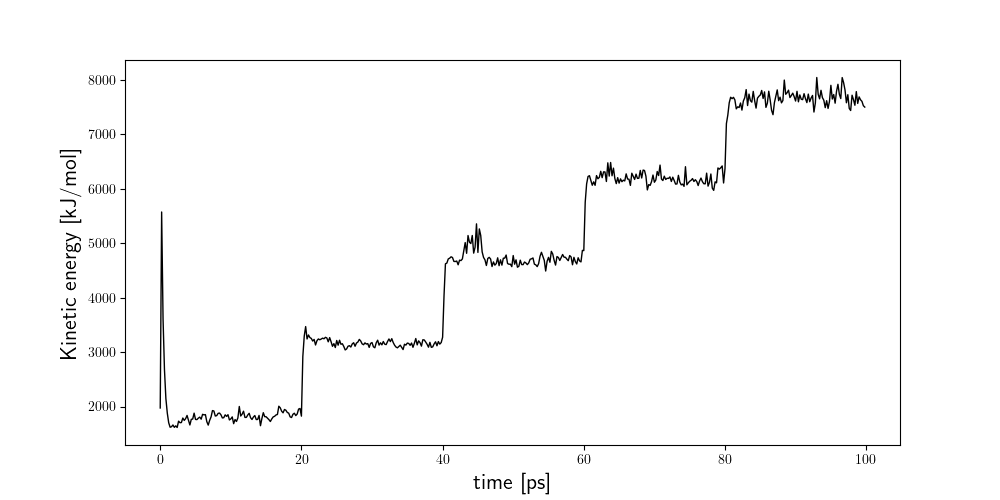
\includegraphics[scale=0.65]{Figures/Chapter_5/totkin.png}
    \caption{The kinetic energy during the equilibration process of the helix penta-alanine.}
    \label{fig:totkin}
\end{figure}




